\documentclass{standalone}
\usepackage{tikz}
\usetikzlibrary{patterns, positioning}


\begin{document}
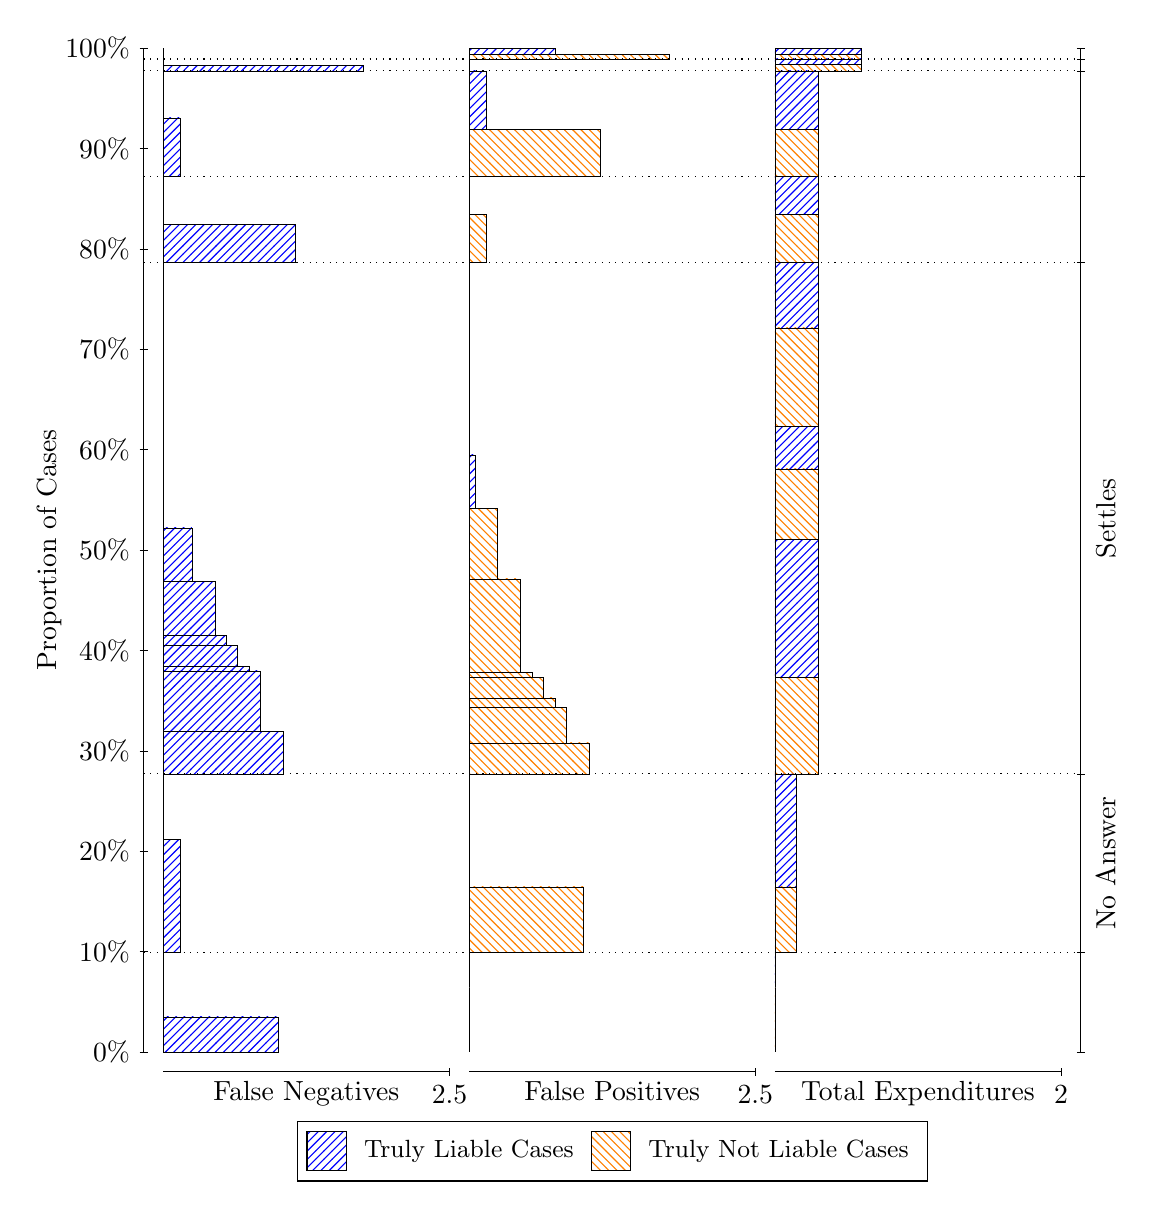
\begin{tikzpicture}
\draw[black, very thin] (1.5,1.75) -- (1.5,14.5);
\node[rotate=90, text=black, anchor=center] at (0.3, 8.125) {Proportion of Cases};
\draw[black, very thin] (1.45,1.75) -- (1.55,1.75);
\node[text=black, anchor=east] at (1.45, 1.75) {0\%};
\draw[black, very thin] (1.45,3.025) -- (1.55,3.025);
\node[text=black, anchor=east] at (1.45, 3.025) {10\%};
\draw[black, very thin] (1.45,4.3) -- (1.55,4.3);
\node[text=black, anchor=east] at (1.45, 4.3) {20\%};
\draw[black, very thin] (1.45,5.575) -- (1.55,5.575);
\node[text=black, anchor=east] at (1.45, 5.575) {30\%};
\draw[black, very thin] (1.45,6.85) -- (1.55,6.85);
\node[text=black, anchor=east] at (1.45, 6.85) {40\%};
\draw[black, very thin] (1.45,8.125) -- (1.55,8.125);
\node[text=black, anchor=east] at (1.45, 8.125) {50\%};
\draw[black, very thin] (1.45,9.4) -- (1.55,9.4);
\node[text=black, anchor=east] at (1.45, 9.4) {60\%};
\draw[black, very thin] (1.45,10.675) -- (1.55,10.675);
\node[text=black, anchor=east] at (1.45, 10.675) {70\%};
\draw[black, very thin] (1.45,11.95) -- (1.55,11.95);
\node[text=black, anchor=east] at (1.45, 11.95) {80\%};
\draw[black, very thin] (1.45,13.225) -- (1.55,13.225);
\node[text=black, anchor=east] at (1.45, 13.225) {90\%};
\draw[black, very thin] (1.45,14.5) -- (1.55,14.5);
\node[text=black, anchor=east] at (1.45, 14.5) {100\%};

\draw[black, very thin] (13.4,1.75) -- (13.4,14.5);
\draw[black, very thin] (13.35,1.75) -- (13.45,1.75);
\node[anchor=west] at (13.35, 1.75) {};
\draw[black, very thin] (13.35,3.0122) -- (13.45,3.0122);
\node[anchor=west] at (13.35, 3.0122) {};
\draw[black, very thin] (13.35,5.281) -- (13.45,5.281);
\node[anchor=west] at (13.35, 5.281) {};
\draw[black, very thin] (13.35,11.777) -- (13.45,11.777);
\node[anchor=west] at (13.35, 11.777) {};
\draw[black, very thin] (13.35,12.865) -- (13.45,12.865);
\node[anchor=west] at (13.35, 12.865) {};
\draw[black, very thin] (13.35,14.21) -- (13.45,14.21);
\node[anchor=west] at (13.35, 14.21) {};
\draw[black, very thin] (13.35,14.361) -- (13.45,14.361);
\node[anchor=west] at (13.35, 14.361) {};
\draw[black, very thin] (13.35,14.5) -- (13.45,14.5);
\node[anchor=west] at (13.35, 14.5) {};

\draw[black, very thin, pattern color=blue, pattern=north east lines] (1.75,1.75) rectangle (3.2033,2.1948);
\draw[black, very thin, pattern color=orange, pattern=north west lines] (1.75,2.1948) rectangle (1.75,3.0122);
\draw[black, very thin, pattern color=blue, pattern=north east lines] (1.75,3.0122) rectangle (1.968,4.4465);
\draw[black, very thin, pattern color=orange, pattern=north west lines] (1.75,4.4465) rectangle (1.75,5.281);
\draw[black, very thin, pattern color=blue, pattern=north east lines] (1.75,5.281) rectangle (3.276,5.8193);
\draw[black, very thin, pattern color=blue, pattern=north east lines] (1.75,5.8193) rectangle (2.9853,6.5896);
\draw[black, very thin, pattern color=blue, pattern=north east lines] (1.75,6.5896) rectangle (2.84,6.6507);
\draw[black, very thin, pattern color=blue, pattern=north east lines] (1.75,6.6507) rectangle (2.6947,6.9105);
\draw[black, very thin, pattern color=blue, pattern=north east lines] (1.75,6.9105) rectangle (2.5493,7.0452);
\draw[black, very thin, pattern color=blue, pattern=north east lines] (1.75,7.0452) rectangle (2.404,7.7263);
\draw[black, very thin, pattern color=blue, pattern=north east lines] (1.75,7.7263) rectangle (2.1133,8.4072);
\draw[black, very thin, pattern color=orange, pattern=north west lines] (1.75,8.4072) rectangle (1.75,11.777);
\draw[black, very thin, pattern color=blue, pattern=north east lines] (1.75,11.777) rectangle (3.4213,12.256);
\draw[black, very thin, pattern color=orange, pattern=north west lines] (1.75,12.256) rectangle (1.75,12.865);
\draw[black, very thin, pattern color=blue, pattern=north east lines] (1.75,12.865) rectangle (1.968,13.613);
\draw[black, very thin, pattern color=orange, pattern=north west lines] (1.75,13.613) rectangle (1.75,14.21);
\draw[black, very thin, pattern color=blue, pattern=north east lines] (1.75,14.21) rectangle (4.2933,14.277);
\draw[black, very thin, pattern color=orange, pattern=north west lines] (1.75,14.277) rectangle (1.75,14.361);
\draw[black, very thin, pattern color=orange, pattern=north west lines] (1.75,14.361) rectangle (1.75,14.424);
\draw[black, very thin, pattern color=blue, pattern=north east lines] (1.75,14.424) rectangle (1.75,14.5);
\draw[black, very thin, pattern color=orange, pattern=north west lines] (5.6333,1.75) rectangle (5.6333,2.5674);
\draw[black, very thin, pattern color=blue, pattern=north east lines] (5.6333,2.5674) rectangle (5.6333,3.0122);
\draw[black, very thin, pattern color=orange, pattern=north west lines] (5.6333,3.0122) rectangle (7.0867,3.8467);
\draw[black, very thin, pattern color=blue, pattern=north east lines] (5.6333,3.8467) rectangle (5.6333,5.281);
\draw[black, very thin, pattern color=orange, pattern=north west lines] (5.6333,5.281) rectangle (7.1593,5.6758);
\draw[black, very thin, pattern color=orange, pattern=north west lines] (5.6333,5.6758) rectangle (6.8687,6.1241);
\draw[black, very thin, pattern color=orange, pattern=north west lines] (5.6333,6.1241) rectangle (6.7233,6.2463);
\draw[black, very thin, pattern color=orange, pattern=north west lines] (5.6333,6.2463) rectangle (6.578,6.5061);
\draw[black, very thin, pattern color=orange, pattern=north west lines] (5.6333,6.5061) rectangle (6.4327,6.5734);
\draw[black, very thin, pattern color=orange, pattern=north west lines] (5.6333,6.5734) rectangle (6.2873,7.7576);
\draw[black, very thin, pattern color=orange, pattern=north west lines] (5.6333,7.7576) rectangle (5.9967,8.6509);
\draw[black, very thin, pattern color=blue, pattern=north east lines] (5.6333,8.6509) rectangle (5.706,9.3317);
\draw[black, very thin, pattern color=blue, pattern=north east lines] (5.6333,9.3317) rectangle (5.6333,11.777);
\draw[black, very thin, pattern color=orange, pattern=north west lines] (5.6333,11.777) rectangle (5.8513,12.386);
\draw[black, very thin, pattern color=blue, pattern=north east lines] (5.6333,12.386) rectangle (5.6333,12.865);
\draw[black, very thin, pattern color=orange, pattern=north west lines] (5.6333,12.865) rectangle (7.3047,13.462);
\draw[black, very thin, pattern color=blue, pattern=north east lines] (5.6333,13.462) rectangle (5.8513,14.21);
\draw[black, very thin, pattern color=orange, pattern=north west lines] (5.6333,14.21) rectangle (5.6333,14.294);
\draw[black, very thin, pattern color=blue, pattern=north east lines] (5.6333,14.294) rectangle (5.6333,14.361);
\draw[black, very thin, pattern color=orange, pattern=north west lines] (5.6333,14.361) rectangle (8.1767,14.424);
\draw[black, very thin, pattern color=blue, pattern=north east lines] (5.6333,14.424) rectangle (6.7233,14.5);
\draw[black, very thin, pattern color=orange, pattern=north west lines] (9.5167,1.75) rectangle (9.5167,2.5674);
\draw[black, very thin, pattern color=blue, pattern=north east lines] (9.5167,2.5674) rectangle (9.5167,3.0122);
\draw[black, very thin, pattern color=orange, pattern=north west lines] (9.5167,3.0122) rectangle (9.7892,3.8467);
\draw[black, very thin, pattern color=blue, pattern=north east lines] (9.5167,3.8467) rectangle (9.7892,5.281);
\draw[black, very thin, pattern color=orange, pattern=north west lines] (9.5167,5.281) rectangle (10.062,6.5061);
\draw[black, very thin, pattern color=blue, pattern=north east lines] (9.5167,6.5061) rectangle (10.062,8.2625);
\draw[black, very thin, pattern color=orange, pattern=north west lines] (9.5167,8.2625) rectangle (10.062,9.1558);
\draw[black, very thin, pattern color=blue, pattern=north east lines] (9.5167,9.1558) rectangle (10.062,9.6941);
\draw[black, very thin, pattern color=orange, pattern=north west lines] (9.5167,9.6941) rectangle (10.062,10.946);
\draw[black, very thin, pattern color=blue, pattern=north east lines] (9.5167,10.946) rectangle (10.062,11.777);
\draw[black, very thin, pattern color=orange, pattern=north west lines] (9.5167,11.777) rectangle (10.062,12.386);
\draw[black, very thin, pattern color=blue, pattern=north east lines] (9.5167,12.386) rectangle (10.062,12.865);
\draw[black, very thin, pattern color=orange, pattern=north west lines] (9.5167,12.865) rectangle (10.062,13.462);
\draw[black, very thin, pattern color=blue, pattern=north east lines] (9.5167,13.462) rectangle (10.062,14.21);
\draw[black, very thin, pattern color=orange, pattern=north west lines] (9.5167,14.21) rectangle (10.607,14.294);
\draw[black, very thin, pattern color=blue, pattern=north east lines] (9.5167,14.294) rectangle (10.607,14.361);
\draw[black, very thin, pattern color=orange, pattern=north west lines] (9.5167,14.361) rectangle (10.607,14.424);
\draw[black, very thin, pattern color=blue, pattern=north east lines] (9.5167,14.424) rectangle (10.607,14.5);
\draw[black, dotted] (1.5,3.0122) -- (13.4,3.0122);
\draw[black, dotted] (1.5,5.281) -- (13.4,5.281);
\draw[black, dotted] (1.5,11.777) -- (13.4,11.777);
\draw[black, dotted] (1.5,12.865) -- (13.4,12.865);
\draw[black, dotted] (1.5,14.21) -- (13.4,14.21);
\draw[black, dotted] (1.5,14.361) -- (13.4,14.361);
\draw[black, very thin] (1.75,1.5) -- (5.3833,1.5);
\node[text=black, anchor=north] at (3.5667, 1.5) {False Negatives};
\draw[black, very thin] (5.3833,1.45) -- (5.3833,1.55);
\node[text=black, anchor=north] at (5.3833, 1.45) {2.5};

\draw[black, very thin] (5.6333,1.5) -- (9.2667,1.5);
\node[text=black, anchor=north] at (7.45, 1.5) {False Positives};
\draw[black, very thin] (9.2667,1.45) -- (9.2667,1.55);
\node[text=black, anchor=north] at (9.2667, 1.45) {2.5};

\draw[black, very thin] (9.5167,1.5) -- (13.15,1.5);
\node[text=black, anchor=north] at (11.333, 1.5) {Total Expenditures};
\draw[black, very thin] (13.15,1.45) -- (13.15,1.55);
\node[text=black, anchor=north] at (13.15, 1.45) {2};


\node[text=black, centered, rotate=90] at (13.72, 4.1466) {No Answer};
\node[text=black, centered, rotate=90] at (13.72, 8.529) {Settles};





\draw (7.449999999999999,1.5) node[draw=none] (baseCoordinate) {};
\begin{scope}[align=center]
        \matrix[scale=0.5, draw=black, below=0.5cm of baseCoordinate, nodes={draw}, column sep=0.1cm]{
            \node[rectangle, draw, minimum width=0.5cm, minimum height=0.5cm, pattern color=blue, pattern=north east lines] {}; &
            \node[draw=none, font=\small, text=black] (B) {Truly Liable Cases}; &
            \node[rectangle, draw, minimum width=0.5cm, minimum height=0.5cm, pattern color=orange, pattern=north west lines] {}; &
            \node[draw=none, font=\small, text=black] (B) {Truly Not Liable Cases}; \\
            };
\end{scope}

\end{tikzpicture}
\end{document}